\documentclass{article}
\usepackage{CJKutf8}
\usepackage{multicol}
% Packages
\usepackage{lipsum} % For generating dummy text
\usepackage[top=1in, bottom=1in, left=1in, right=1in]{geometry}
\usepackage{hyperref}
\usepackage{pgfplots}
\usepackage{caption}
\pgfplotsset{compat=1.17} % Use this to ensure compatibility with newer features
\setlength{\parskip}{6pt}
% Title and author
\title{Autonomous competence identification protocol}
\author{Tim Pechersky}


\begin{document}
\begin{CJK}{UTF8}{gbsn}

\maketitle



\begin{abstract}
    This paper proposes a novel protocol for designing ranking systems applicable to consensus-building protocols and decentralized autonomous organizations (DAOs). Leveraging recent cryptographic advancements and social science insights, the protocol facilitates autonomous decision-making in trustless environments based on agent interactions, addressing key challenges in autonomous organizations. We examine an existing precedent, originating as an easy-to-understand tabletop game, which demonstrates promising participation rates even among non-technical users. Our proposed implementations focus on defining interoperable and liquid voting weights for participants, facilitated in both computational and non-computational (social) networks. Additionally, we briefly review economic models for the practical utilization of such competence frameworks and game theoretic moments.
\end{abstract}
\begin{multicols}{2}

\section{Introduction}

The quest for consensus, a cornerstone of collective decision-making, has deep historical roots. From the ancient Chinese concept of \textit{zhongyong} {\CJKfamily{bsmi}
中庸}, advocating for moderation and balance in governance, to the Roman Republic's emphasis on \textit{senatus consulta} (senate decrees) reached through deliberation and compromise, societies have long grappled with the challenge of aligning diverse perspectives towards a common goal. The study of these historical precedents continues to inform modern approaches to consensus \cite{Andersen2019} \cite{Frederic2014}. \\
The pursuit of consensus, has gained renewed significance in the digital age. Originating from the Bitcoin whitepaper \cite{Satoshi}, blockchain technology fundamentally seeks consensus and establishes trustless systems through cryptographic signatures. While significant progress has been made in developing efficient Byzantine Fault Tolerance (BFT) algorithms for reaching consensus on verifiable data \cite{Genrui2023}, the challenge of achieving consensus on subjective or non-deterministic matters within DAOs \cite{Hassan2021} remains a complex issue \cite{Shuai2019}\cite{Rainer2023}. This has led some researchers to question the ability of autonomous organizations to overcome the hierarchical issues present in today's society \cite{Marcella2016} \cite{Xuan2024}.   \\
This paper addresses the gap between formally verifiable, automated consensus and subjective human decision-making. We propose a protocol that can achieve consensus even for subjective matters by qualifying participants based on their ability to represent a group's interests and intents. This protocol aims to provide a foundational building block for designing ranking systems applicable to both computational and social networks, and capable to address some of long standing governance issues such as agenda manipulation \cite{McKelvey1976} problem.\\
Main objectives thus are to propose a methodology for creating a ranking system in a trustless environment, review attack vectors and resistance mechanisms, provide a case study of existing use-case and discuss potential economic models for the practical utilization of such competence frameworks.
We begin by reviewing existing consensus mechanisms and their limitations, focusing on DAOs and their governance mechanisms. We then introduce our proposed protocol, followed by a discussion of its implementation and potential economic models. Finally, we present a case study of an existing use case and conclude with a discussion of future research directions.\\

\section{Background}
% Write your methodology here
Decentralized Autonomous governance nor consensus protocols can be defined trough cyber-physical systems \cite{Lee2008} methodology completely, nevertheless ultimately is an end goal for any autonomous governance is to operate CPS. In this context any kind of IT governance system can be seen trough methodology of Cyber-Physical-Social-System (CPSS) \cite{Fei2016}.


Studies of management perspectives in cyber age introduce parallel management \cite{Wang2022} ideas, management frameworks proposed to model DAOs as CPSS openly discuss need for multidimensional indexes and foundational models \cite{Juanjuan2023}. In order to support such grand design ambition, the DAO organizations must be able to show other metrics of their governance to provide the best possible performance. Additionally, as discussion for parallel management \cite{Wang2022}, there is a need for a robust mechanism for reinforcing the informational and intellectual capabilities of organizations, enabling them effectively benchmark performance of AI enabled agents against human in various tasks and aspects of governance and management.

In order to support quantities analysis of decentralization metric, Nakamoto Coefficient\cite{Balaji2017} was proposed, defined as \textit{how many entities one would need to to be compromised to control entire system} it can be used as decentralization criteria.

Besides these new concepts, the traditional governance models long standing problems, such as agenda manipulation \cite{McKelvey1976} that should be addressed well to ensure high reliability of organizations in autonomous systems.


\subsection{Consensus Layer}
Blockchain is a distributed and decentralized network that follows some particular consensus protocol in order to maintain continuous sequence, chain of blocks\cite{Merlinda2019}, where each new block consists of a digital records to a united ledger book. First introduced at launch of Bitcoin\cite{Satoshi}, since then grown to an industry where multiple approaches and protocols were developed and initial ability to write a records in to ledger book was elaborated to ability to write code in ledger records such that can change states of book itself.
The blockchain governance plays a critical role in any blockchain protocol and can be summarized as consisting of Validators, Users, Governance Mechanisms and core developer community; In this context blockchain network is analogous to an organization, consisting validators (employees), protocols and governance structure whose activity result in services provided to users that also have to say their word by paying for using the protocol.

The contrast between traditional organization and blockchain governance is CSP friendly automation. Such are designed to follow some determined rules of maintaining distributed ledger with no need for human stakeholder decision for a regular operations which are automated by running specific software applications (nodes) that act on behalf of stakeholder.
These however work only well up to the point when the protocol changes are desired or some vulnerability happens which leads to stakeholder collective decision for stepping-off the protocol rules \cite{Liu2021} for at least one block. Such occasions generally are called hard-forks and have specifics that coordinated consensus between node operators changes their protocol rules to move away from existing logic. The "fork" in context describes split of consensus in two possible ledger book states which are not compatible. \\
Consensus layer protocols also have the underlying node operator community which incentive driven and studies on Nash Equilibrium \cite{Nida2020} are done while the real situation for Ethereum is that Miner Extracted Value is shown \cite{Philip2019} as realistic thread to protocol level security that comes down to affecting applications such as decentralized exchanges. Same paper also observes that agents pursuing MEV can achieve cooperative equilibrium in terms of priority gas auctions. \\
"Ethereum Proof-of-Stake Consensus Layer: Participation and Decentralization research" \cite{Dominic2023} has shown that practical Nakamoto coefficient numbers in automated consensus engines such as PoS and Pow (Proof of Stake and Work accordingly) have stabilized on a very low numbers of less then 5 entities standing behind whole pool of validators and miners, and seem not to show any positive dynamics.


\subsection{Application Layer}
While research in CPSS field point out demand for DAOs as solution \cite{Fei2016}\cite{Wang2022}\cite{Juanjuan2023}, the ability of DAOs to perform well and be competitive, however, is under question, as many research point out associated problems \cite{Rainer2023}\cite{Marcella2016}\cite{Xuan2024}.  \\An empirical Study of On-Chain Governance conducted by Rainer Feichtinger et. al. \cite{Rainer2023} shows low Nakamoto coefficient numbers, however comparing it with Consensus Layer research \cite{Dominic2023} we can conclude there is a positive dynamic in the Nakamoto coefficient over time in DAOs, compared with absence of such for the consensus layer. Same research\cite{Rainer2023} also shown that analyzed DAOs Gini coefficients\cite{Lidia2012} are high, reaching 0.888-1 for direct holders and 0.667-0.980 range when counting delegates, also shown participation rate in DAOs are low. Out of four analyzed DAOs (Compound, Uniswap, ENS and Gitcoin), none of them are showing positive dynamics in participation rate over time, and mean numbers for participation even amongst delegates are in range of 1.1-9.9\% of total delegated accounts.


Another highlighted problem can be seen in the voting participation rates, which are low. For example, Compound DAO quorum requires only 400,000 \cite{CompDAO} votes out of 10,00,000 total token supply \cite{CompToken}, which is only 4\%, yet in practice some of proposals fail to reach even this low threshold from the first time and have to re-submit \cite{CompProp232}\cite{CompProp237}. To illustrate problem further some quorum requirements are illustrated in Table \ref*{table:dao-metrics}. Such low quorum requirements are directly explainable by a low participation rates, and already have a record of quorum attacks \cite{AragonBlog}\cite{rhizoo2023} precedents, that were exploiting this weakness, while contrary in high participation rate consensus layer systems, such as PoS and PoW, the financial incentives towards participation shown not just to negatively impact  Nakamoto coefficients, but also have shown that any network node must be seen as rational-agent which may diverge from collective interest \cite{Philip2019}.

\end{multicols}
\begin{table}[ht]
    \centering
    \caption{DAO Minimal Quorums}
    \label{table:dao-metrics}
    \begin{tabular}{|l|l|l|l|}
    \hline
    \textbf{Name of DAO} & \textbf{Total Supply} & \textbf{Quorum} & \textbf{Threshold (\%)} \\ \hline
    Compound             & 10e6            & 400e3             & 4\%                     \\ \hline
    Uniswap              & 1e9             & 40e6              & 4\%                     \\ \hline
    ENS                  & 100e6           & 1e6               & 1\%                     \\ \hline
    Arbitrum             & 10e9            & 300e6-500e6       & 3-5\%                   \\ \hline
    Lido                 & 1e9             & 50e6              & 5\%                     \\ \hline
    \end{tabular}
    \end{table}
\begin{multicols}{2}

\subsection{Comparing two above}
DAOs ultimately are just an abstraction layer on top of Consensus, allowing blockchain users to abstract away from calculations intensity onto smart contract programming and therefore more versatile, dynamic governance systems that can rely on underlying consensus security guarantees. Difference however also lies in implementation specifics: while Consensus layers do provide participation incentives, the application layer organization might not propose such at all, instead providing a means to make a governance decisions that are profitable on their own. \\ Analyzing  Nakamoto coefficient we can see a notable difference between Nakamoto coefficient in DAOs vs Consensus layer. One possible explanation for this phenomenon can be coined as "curse of money making money". It suggests that in order to ensure growth of Nakamoto coefficient, the ability to influence the system should grow at a rate that must be sub-linear in relation to entities efforts (investments), ensuring that no disproportionate compounding of power occurs. In other words, the growth of influence should not match or exceed a linear rate to prevent centralization, highlighting the necessity for mechanisms that enforce a diminishing increase in influence relative to investment or contribution (Fig. \ref*{fig:growth-influence}).

One another notable difference is in the security model. While relying on consensus engine enables security guarantees, the opposite side of that medal is that such application layer governance mechanisms have no similar alternative as consensus layer operators do with hard-fork ability. Even if community members agree on such decision in case exploit happens, there is no easy way to "split away" saving full state. The only known occasion of such successful split was The DAO Hack Hard-fork which was done very controversially at the protocol level.  \cite{Liu2021}.
This is a substantial difference with consensus layers, where any participation requires a commitment that either requires to do work prior to a particular vote (PoW), or have assets at stake (PoS, Optimistic Rollups) that can be lost during due to any activity by operator against the protocol rules.\\
Lack of such ongoing commitment mechanisms in the application layer, brings in substantial security risks as governance attacks become less risky for the adversary \cite{AragonBlog}\cite{rhizoo2023}. Such risks led to solutions such as time-locks \cite{Jack2021}, and rage quit \cite{Ameen2019} methods giving individual stakeholders a last-resort options to leave the protocol (arguably) safely at the expense of delayed actions taken by the organizations.

While these solutions are effective in preventing funds loss, the reduce in reaction time by organization is not always acceptable. Need for prompt decision making is leads to empowering security players to run a privileged multi-signature wallets to run emergency stop or veto power over DAO protocols \cite{Jason2024}. Fact of presence of such, centralizing actors makes DAO frameworks to behave in non-autonomous way. The more general question is left open - how to appoint such privileged actions takers in an autonomous ways, ideally defining the privileges as a function of certainty in the actor?

\end{multicols}
% Manually place the figure without the figure environment
% Inside the multicol environment

\begin{figure}[ht]
    \centering
    \begin{minipage}{0.45\textwidth}
        \centering
        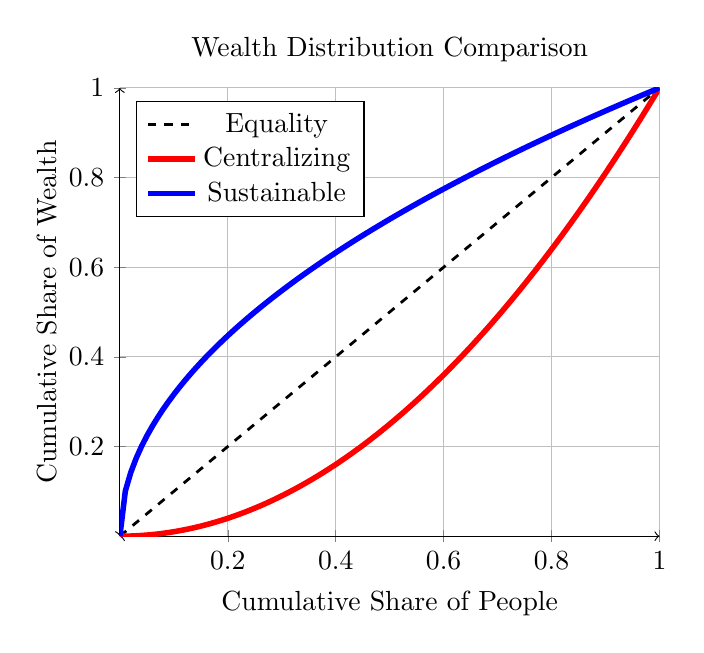
\begin{tikzpicture}
            \begin{axis}[
                title={Wealth Distribution Comparison},
                xlabel={Cumulative Share of People},
                ylabel={Cumulative Share of Wealth},
                xmin=0, xmax=1,
                ymin=0, ymax=1,
                legend pos=north west,
                axis lines=middle,
                axis line style=<->,
                x label style={at={(axis description cs:0.5,-0.1)},anchor=north},
                y label style={at={(axis description cs:-0.1,.5)},rotate=90,anchor=south},
                grid=major,
                ]
                % Line of Equality
                \addplot[
            color=black,
            mark=none,
            dashed,
            line width=1pt,
            domain=0:1,
            ]{x};
        \addlegendentry{Equality}

        % Centralizing Incentives Lorenz Curve
        \addplot[
            color=red,
            mark=none,
            line width=2pt,
            domain=0:1,
            samples=100,
            ]{x^2};
        \addlegendentry{Centralizing}

        % Sustainable Incentives Lorenz Curve
        \addplot[
            color=blue,
            mark=none,
            line width=2pt,
            domain=0:1,
            samples=100,
            ]{sqrt(x)};
        \addlegendentry{Sustainable}

        \end{axis}
        % Your first plot code here
        \end{tikzpicture}
        \caption{First Plot}
        \label{fig:growth-influence}
    \end{minipage}\hfill
    \begin{minipage}{0.45\textwidth}
        \centering
        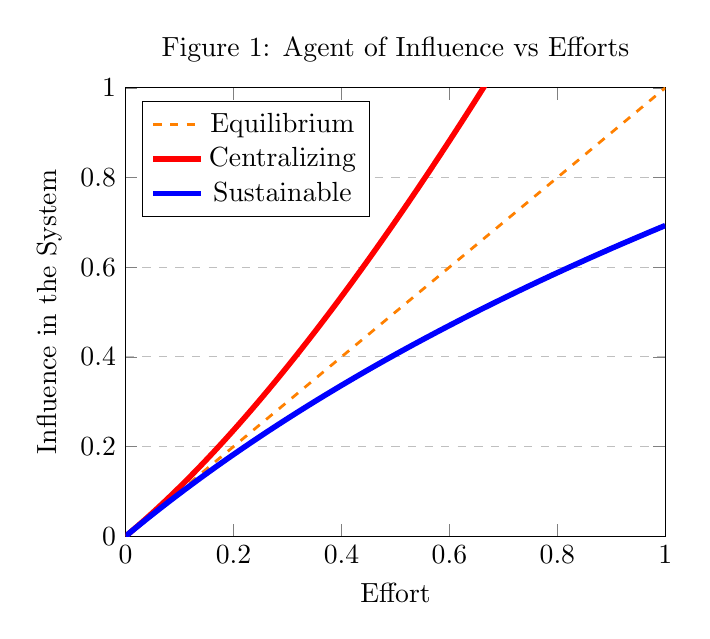
\begin{tikzpicture}
            \begin{axis}[
                title={Figure 1: Agent of Influence vs Efforts},
                xlabel={Effort},
                ylabel={Influence in the System},
                xmin=0, xmax=1,
                ymin=0, ymax=1,
                legend pos=north west,
                ymajorgrids=true,
                grid style=dashed,
            ]
            % Linear growth
            \addplot[
                color=orange,
                mark=none,
                dashed,
                line width=1pt,
                domain=0:1,
                ]{x};
            \addlegendentry{Equilibrium}
            % Sub-linear growth (example: square root)
            \addplot[
                color=red,
                mark=none,
                line width=2pt,
                domain=0:1,
                samples=100,
                ]{x+x*(ln(x+1))};
            \addlegendentry{Centralizing}
            \addplot[
                color=blue,
                mark=none,
                line width=2pt,
                domain=0:1,
                samples=100,
                ]{{ln(x+1)}};
            \addlegendentry{Sustainable}
            \end{axis}
        % Your second plot code here
        \end{tikzpicture}
        \caption{Second Plot}
    \end{minipage}
\end{figure}
\begin{multicols}{2}

\subsection{Recent cryptographic advancements}
Recent cryptographic advancements have enabled the development of new governance and consensus mechanisms that may be used to address the challenges faced by DAOs. For example, the use of zk-SNARKs (Zero-Knowledge Succinct Non-Interactive Argument of Knowledge) allows for the creation of verifiable and private voting systems that can be used to ensure the integrity of voting processes within DAOs \cite{Ben-Sasson2014}, while MPC threshold-signature protocols can be used to create secure multi-party data signing process \cite{Doerner2023} and fully homomorphic encryption promises us soon ability to run fully private calculation directly on-chain \cite{Fhenix}.\\
Summing this section up, we can say that whatever new protocol is designed for governance, it is realistic to set requirements of privacy in voting and proposing process.

\subsection{Proposed Protocol origins}\label{sec:protocol_origins}
Foundation for this research originates from existing precedent of a game that is played by small Lithuanian group of friends in chat messenger since 2017. This original game never had ambition to become a protocol or a system, but it was a fun way to spend time and exchange music ideas between friends-musicians who were all living in different countries and used it as mean to stay engaged. The game typically consists of 5 to 10 people, and series of rounds. Each round a player is assigned a role of a "game master". Participants send game master music compositions they like and game master compiles them into a playlist. The playlist is then shared with all participants, who vote on their favorite composition by sending their vote to the game master again. At the end of a turn, the game master reveals the proposer identities, as well as scores proposal based on votes. The game continues to the next round until total of hundred compositions are added to the playlist. Each round scores are aggregated per participant, yielding a final ranking.\\
Notably, the game has high agenda manipulation resistance, as every participant is required to make a proposal, in order to vote, which is contrary to traditional voting systems, where small group of proposers can pose a threat  \cite{McKelvey1976}. Also this game mechanics effectively coupes negative effects of proposals such as known as Hallo effect \cite{Verhulst2010}. \\
It also demonstrates some of the key features that are desirable in a governance protocol, such as high participation rates, user retention, while the only limit is that participants generally may be interested to participate only in the specific field (music) or with a specific group of people.

It appears that participants in order to conduct a round must \(i\) submit a proposal, \(ii\) get proposals batch, \(iii\) submit a vote, resulting communication complexity $O(3n)$ per round


\subsection{Summing up the problem}

\section{Protocol Description}
From the issues identified in the background sections we can sum up that there are multiple problems that are faced both on network protocol level governance as well as on application layer built DAOs as well: Low participation rates, low Nakamoto coefficients, lack of application layer commitments, and lack of multidimensionality.
We can also note that incentive based protocols cause centralization, yet decentralized organizations are not able to provide a commitment mechanism for participants, nor do they have autonomous way to automatically identify competent actors in the system to take prompt, time-critical actions.\\
We have discussed two different kinds of systems so far - based on consensus layer continuous proving and application layer share-holder voting and identified different problems of both of these kinds. \\
Assuming there can be some kind of general solution for these, we can outline a generic DAO specifications, we are looking for a protocol that will enable a generic DAO to have following properties:\\
\textbf{High participation rates}: The protocol participants should actively participate in the decision-making process by the design of the protocol, not by the external incentives.\\
\textbf{Resistant to influence compounding}: Protocol should be designed in a way that over time dependency on single actors shall be reduced, Nakamoto coefficient shall grow.\\
\textbf{Application layer commitments}: Protocol should allow DAO to require participants to make a commitment to the organization in order to participate in the decision-making process.\\
\textbf{Multidimensionality}: Protocol should enable multidimensional indexes and foundational models to be built on top of it, as well as promote working groups that can be more operative than a main governing body.\\
\textbf{Rational agent friendly}: Protocol should be designed in a way that any network node must be seen as rational-agent which may diverge from collective interest or collude with others and still not able to reach  influence over the system beyond what protocol accounts for.



Based on provided background section for protocol origins, In order to support solving all of the objectives, we can specify that outcome of protocol is a transferrable asset, that represents competence of the participant in a particular subject. This subject may be represented as a string of text, describing it, or as a URI to a resource that describes it.
Transferability is an important aspect as this allows us to account agent rational actions, and even high concepts of corruption and collusion, as a free-market values that are not necessarily bad and simply define intrinsic value of any transferable asset. Other words saying, we see personal competences in CPSS frameworks useful as a market value, that can be traded. While this can me argued as a controversial statement, we can see that in the real world, the competence is often traded in form of a investing time and money in education, and since we declare as a requirement to have a compounding resistance, we can see that this is a way to ensure that the competence is not traded in a way that it can be easily bought by a single entity. Similarly intrinsic value can be used by organizations that use protocol to define staked commitments, similarly as PoS consensus mechanisms do.\\
Subjects themselves provide a way to ensure multidimensionality, for example a text string may be vectorized with Large-Language-Model to provide a multidimensional representation of the subject, or a URI may be used to point to a resource that provides a multidimensional representation of the subject.\\
Free market economy already discussed in this section will just help to arbitrage between different successful and largely adopted subjects that share same dimensionality.
Providing a influence to compounding becomes a critical aspect part for such protocol, since we are relying to a free-market values and principally do not require any specific identity solution as a dependency to this protocol.
Our foundational model for this resistance lies in extending  ~\ref{sec:protocol_origins} idea, to introduce \textit{ranking ladder} that lets game winner to participate in next game with higher level of rewards, this expected to create non-linear friction towards any sybil attack, allowing competent actors who are willing spend their time to participate in the game to be rewarded with advantage over any colluding company that is trying to game the system.
This requirement leaves us to the last, but not least requirement: High Participation rates.
We argue that multidimensionality and free-market values will provide a way to ensure high participation rates, as participants will be able to participate in the decision-making process in a category that they are interested in, and that they are competent in, and lastly - are rewarded for being in.
With a ranking ladder, and a multidimensional representation, this can be seen as a global framework for building education and helping young talents to discover their path by observing very well quantized data on their progress. We also suggest that this protocol foundational should be presented as simply a new way of talking, where each input - seen as valuable idea, and each vote - seen as a valuable feedback, and each game final, as actionable result.\\
that is multiple participants are required to support a winner.


% Write your conclusion here
\section{Implementation}
Protocol particular implementation may vary depending on environment and requirements, however we can outline a generic implementation that can be used as a reference for further development.\\
The protocol can be implemented as a smart contract on a blockchain network, such as Ethereum, that allows participants to submit proposals, vote on proposals, and receive rewards based on their participation. Subject representing subject asset can be represented as semi-fungible asset, like ERC1155\cite{EIP1155} standard interface on Ethereum, where each token id represents a rank level, and games that award such rank require a token of one below to be held in order to participate. Such token shall be created only as a result of competence identifying smart contract activity result. The competence identifying contract is a turn-based game where group must collect together and has a signer-key (game master), who is able to sign for a private inputs and keep personalities of participants hidden by either using MPC or zk-SNARKs protocol.
The game master is responsible for collecting proposals and announcing fact of activity without disclosing the actor, then posting them as batch to a contract, collecting votes in a similar manner, without tell nor who, nor for whom votes, and finally revealing the results.\\



% Write your results here
\section{Case Study}
Some rough statistical data could be gathered by analyzing groups activity and historical records, which show that since 2017 total 17 games were played up to end of 2023. Each averaged for 13 turns, 8 participants and 3 month duration. Total amount of proposals and votes reaching ~1700, as game is stopped at 100 songs playlist length. Total 34 participants joined it over course of years, out from which 22 players completed at least one full tournament and 15 completed at least two full tournaments. From original 6 players 3 still were playing at the moment of writing, with active user count 8 at latest game, showing steady with high user retention. Total amount of players not submitting a vote shown to be negligibly small, below 5\% of all votes. \\
Even despite absence of any incentives beyond that participants are genuinely interested in the subject, and burden of having to be a game master occasionally which requires participants to do some effort, we can see exceptionally high user participation rates with average:
\begin{itemize}
    \item participation rate of 95\% for active users
    \item User retention for three month period of 65\%
    \item User retention for two tournaments and roughly six month of 44\%
    \item User retention after 72 month of 9\%
    \item Average of 8 proposals and votes per participant per annum
\end{itemize}

The low absolute numbers however are explainable by user complex manual score calculation process and closed community by itself which never oriented itself towards big growth and hence let to do assertion that could be even higher on a well designed automated protocol.

We also observed that collected playlists, ordered by high-score compositions, are of high quality and form a good representation of participants' preferences, while the winner of the tournament is often a participant that is able not simply propose a popular song, but to propose a song that is liked by many participants, including such aspects that participants will likely vote songs they hear for the first time (original ideas).

\section{Conclusion}

\end{multicols}{2}
we are generalizing the proof based consensus mechanisms for social network interaction by viewing any network node as rational-agent which may diverge from collective interest \cite{Philip2019} individually or collude with others. We propose BFT tolerance methodology that allows reaching effective consensus based on participant inputs, opinions and  we can say that protocols reach an agreement in a trustless environment by qualifying the competence of the participants. Bitcoin miners are required to solve a cryptographic puzzle to prove their competence, or ethereum Proof of Stake consensus mechanism qualifies participants by their ability by ability to adhere to distributed ledger rules a   nd stake their assets. \\ Similarly DAO participants are qualified by their ability to hold a token and participate in the voting process. Tokens held can be seen as analogy to stake in PoS consensus mechanism, incentivising participants to act in the best interest of the organization. The gap however exists between such automated protocols and DAO governance as organizations agenda may be much more arguable then a "simple" cryptographic puzzle, which despite any computational complexity it might have, most of the time can be formally verified to be correct.\\
This becomes more emergent as the DAOs are becoming more complex and must take effective and prompt decisions in a trustless environment, which often leads to burden of complexity on users, while often a decision making process involves a fairly traditional board-level discussions within governance forum boards, which yields for doubts as researchers find blockchain-based governance systems likely not to solve problems of social.

The contrast between traditional organization and blockchain is that latter are set to follow some determined protocol of following consensus layer decisions in an autonomous way, therefore enabling CPS, there is no need for human stakeholder decision for a regular operations which are automated by running specific software applications (nodes) that maintain protocol on behalf of stakeholder.
These however work only well up to the point when the protocol changes are desired or some vulnerability happens which leads to need for stepping-off the protocol rules for at least one block. Such occasions generally are called hard-forks and have specifics that coordinated consensus between node operators changes their protocol rules to move away from existing logic. The "fork" in context describes split of consensus in two possible ledger book states which are not compatible.
\bibliographystyle{ieeetr}
\bibliography{whitepaper.bib}

\clearpage\end{CJK}
\end{document}